\documentclass[12pt,letterpaper]{article}
\usepackage[utf8]{inputenc}
\usepackage{amsmath,amssymb,fullpage,graphicx}
\usepackage{subfigure}
\usepackage{amssymb}
\let\hat\widehat
\let\tilde\widetilde


\author{Nan Tang\\1662478}
	%% your name
\title{STAT 403 Spring 2018\\HW03}
	%% title of this document
\begin{document}
\maketitle
	%% make the title and author

\section*{Q1}

\subsection*{Q1-a}

\begin{verbatim}
data("chickwts")

feed_linseed_dt <- subset(chickwts, feed == 'linseed')

> t.test(x=feed_linseed_dt, mu=240, alternative='two.sided')

	One Sample t-test

data:  sample_wt
t = -1.4092, df = 11, p-value = 0.1864
alternative hypothesis: true mean is not equal to 240
95 percent confidence interval:
 185.561 251.939
sample estimates:
mean of x 
   218.75 
\end{verbatim}

\noindent We can perceive from summary that the p-value calculated from our sample is 0.1864, which is greater than 0.1. Therefore, under the test size $\alpha = 0.1$, we cannot reject the null hypothesis.\\

\newpage
\subsection*{Q1-b}

\begin{verbatim}
> mean(feed_linseed_dt$weight)
[1] 218.75
> sd(feed_linseed_dt$weight)
[1] 52.2357
\end{verbatim}

\noindent Mean weight of chicken fed by linseed is 218.75 \\
Standard deviation is 52.2358 \\

\subsection*{Q1-c}
\begin{verbatim}
sim_size <- 10000
alpha <- 0.1
sim_result <- rep(NA, sim_size)
for (i in 1:sim_size) {
  sample <- rnorm(n=12, mean=220, sd=52)
  t_result <- t.test(x=sample, mu=240, alternative='two.sided')
  sim_result[i] <- t_result$p.value < alpha
}
t_power <- sum(sim_result) / sim_size

> t_power
[1] 0.3377
\end{verbatim}

\noindent The power of the t-test under the condition that true population mean is 220, is the probability of rejecting $H_0$: $\mu_0 = 240$ with test size $\alpha = 0.1$ . \\

\noindent Base on my simulation, 3377 of 10000 simulations rejected the null. Since the proportion of rejection among simulations is an unbiased estimator of test power, we can say the power of t-test under this condition is $\frac{3377}{10000} = 0.3377$.

\newpage
\subsection*{Q1-d}
\begin{verbatim}
sim_size <- 10000
sample_sz_seq <- c(12,24,36,48,60,72,84,96)
power_seq <- rep(NA, length(sample_sz_seq))

for (i in 1:length(sample_sz_seq)) {
  sim_result <- rep(NA, sim_size)
  for (j in 1:sim_size) {
    sample <- rnorm(n=sample_sz_seq[i], mean=220, sd=52)
    t_result <- t.test(x=sample, mu=240, alternative='two.sided')
    sim_result[j] <- t_result$p.value < alpha
  }
  t_power <- sum(sim_result) / sim_size
  power_seq[i] <- t_power
}

size_power_comp <- data.frame(cbind(sample_sz_seq, power_seq))
colnames(size_power_comp)[1] <- 'size'
colnames(size_power_comp)[2] <- 'power'

col_ramp = colorRampPalette(c("skyblue","limegreen"))

plot(x=size_power_comp$size, y=size_power_comp$power, col=col_ramp(nrow(size_power_comp)),
     pch=20, cex=2, xlim=c(10, 100), main='Size-Power Plot (test size 0.1)', 
     ylab='Power of t-test', xlab='Sample Size')
lines(x=size_power_comp$size, y=size_power_comp$power, lwd=3, col="skyblue")
grid(nx=NA,ny=NULL,lty=1,lwd=0.5,col="gray")
\end{verbatim}

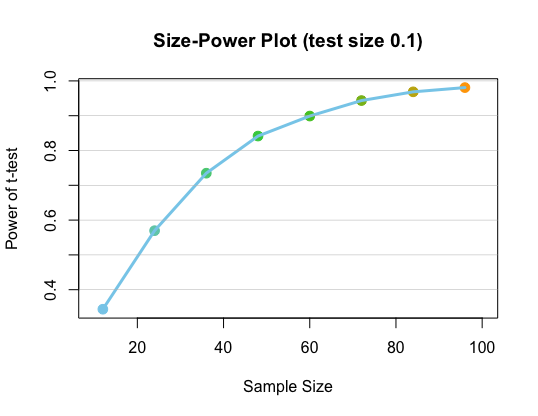
\includegraphics[width=150mm]{size-power.png}

\noindent Under the condition of same true parameter and same test size, the power of t-test has a logarithmic  growth as sample size increases. 

\subsection*{Q1-e}
\noindent When estimating the power of test, the variance of Monte Carlo  simulation is

\begin{align*}
Var(\bar{D}_N) = \frac{\beta (1 - \beta)}{N}
\end{align*}

\noindent $N$ denotes number of simulations, $\beta$ is power of t-test. Under the same sample size and test size, the power is constant.  \\

\begin{align*}
Var(\bar{D}_{N=10000}) &= \frac{\beta (1 - \beta)}{10000}  \\
Var(\bar{D}_{N=1000000}) &= \frac{\beta (1 - \beta)}{1000000} \\
\frac{Var(\bar{D}_{10000})}{Var(\bar{D}_{1000000})} &= 100
\end{align*}

\noindent Thereby we know that the Monte Carlo Variance of 10000 simulations is 100 times larger than error of 1000000 simulations. The Monte Carlo error is $sd(\bar{D}_N) = \sqrt[]{Var(\bar{D}_N)}$, therefore, error of $N=10000$ is $\sqrt[]{100} = 10$ times bigger than error of $N=1000000$\\

\noindent We assumed the Monte Carlo error at N = 10000 is $5 \times 10^{-3}$, therefore, the error of Monte Carlo simulation with N = 1000000 will be $5 \times 10^{-4}$.

\section*{Q2}
\subsection*{Q2-a}

\begin{verbatim}
sim_size <- 10000
sample_size <- 50
minunif_eva <- rep(NA, sim_size)

for (i in 1:sim_size) {
  sample <- runif(sample_size)
  minunif_eva[i] <- min(sample)
}
> mean(minunif_eva)
[1] 0.01959125
> sd(minunif_eva)
[1] 0.01923361
\end{verbatim}

\noindent Mean of $M_{50}$ is 0.01959125 \\
Standard deviation of $M_{50}$ is 0.01923361\\

\newpage
\subsection*{Q2-b}
\begin{verbatim}
x_value <- seq(from=0, to=max(minunif_eva), by=0.001)
exp50 <- dexp(x_value, 50)

hist(minunif_eva, breaks=50, col='skyblue', probability=T, 
     main='Histogram of M50 with Exponential(50)', xlab='M50')
lines(x=x_value, y=exp50, lwd=3, col='purple')
grid(nx=NA,ny=NULL,lty=1,lwd=0.5,col="gray")
legend('right', legend='Exp(50)',
       col='purple', lty=1:2, cex=0.8)
\end{verbatim}

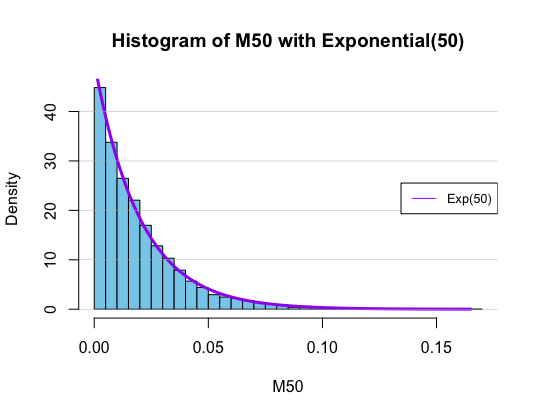
\includegraphics[width=150mm]{hist-exp50.png}

\noindent The distribution of $M_{50} = Min(U_1, U_2, ... U_{50})$ seems to fit the density curve of $exp(50)$.

\newpage
\subsection*{Q2-c}
\begin{verbatim}
sample_size <- 100
minunif_eva <- rep(NA, sim_size)

for (i in 1:sim_size) {
  sample <- runif(sample_size)
  minunif_eva[i] <- min(sample)
}

x_value <- seq(from=0, to=max(minunif_eva), by=0.001)
exp50 <- dexp(x_value, 100)

hist(minunif_eva, breaks=50, col='#b2df8a', probability=T, 
     main='Histogram of M100 with Exponential(100)', xlab='M100')
lines(x=x_value, y=exp50, lwd=3, col='#1f78b4')
grid(nx=NA,ny=NULL,lty=1,lwd=0.5,col="gray")
legend('right', legend='Exp(100)',
       col='#1f78b4', lty=1:2, cex=0.8)
\end{verbatim}

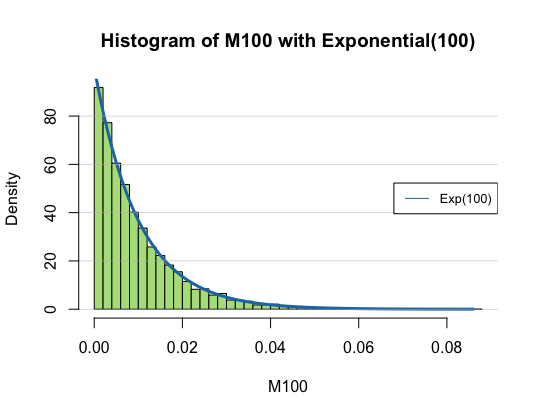
\includegraphics[width=150mm]{hist-exp100.png}

\noindent The distribution of $M_{100} = Min(U_1, U_2, ... U_100)$ seems to fit the density curve of $exp(100)$.

\newpage
\subsection*{Q2-d}

\noindent Find the cdf of $nM_n$
\begin{align*}
P(nM_n \geq x) &= P(M_n \geq \frac{x}{n}) \\
&= P(U_1 \geq \frac{x}{n}, U_2 \geq \frac{x}{n}, ... U_n \geq \frac{x}{n}) \\
&= P(U_1 \geq \frac{x}{n})P(U_2 \geq \frac{x}{n}) ... P(U_n \geq \frac{x}{n}) \\
&= (1 - P(U_1 < \frac{x}{n}) ) (1 - P(U_2 < \frac{x}{n}) ) ...  (1 - P(U_n < \frac{x}{n}) ) \\
&= (1 - F_U(\frac{x}{n}))^n,  (F_U(\frac{x}{n}) = \frac{x}{n}) \\
&= (1 - \frac{x}{n})^n
\end{align*}

\begin{align*}
F_{nM_n}(x) &= 1 - P(nM_n \geq x) \\
&= 1 - (1-\frac{x}{n})^n 
\end{align*}

\noindent The exponential function tells us that 
\begin{align*}
\lim_{n\to\infty}(1 + (-\frac{x}{n}))^n = e^{-x}
\end{align*}
\noindent As n goes to infinity, the cdf and pdf of $nM_n$ turn out to be
\begin{align*}
\lim_{n\to\infty} F_{nM_n}(x) &= 1 - e^{-x} \\
\lim_{n\to\infty} f_{nM_n}(x) &= \frac{\partial F_{nM_n}}{\partial x} \\
&= e^{-x}
\end{align*}
\noindent The pdf of $Exp(1)$ is also defined as $\epsilon (x) = e^{-x}$, therefore, 
\begin{align*}
\lim_{n\to\infty} f_{nM_n} &= e^{-x} = \epsilon (x)
\end{align*}
\noindent This proves that as $n$ goes to infinity $n \cdot M_{n}$ converses in distribution to $exp(1)$.


%%% do not touch anything below
\end{document}
